% !TEX root = ../my-thesis.tex
%
%\selectlanguage{english}  
\chapter{An ontological system based on MODIS images to assess ecosystem functioning of Natura 2000 habitats: A case study for \Qp forests}\label{sec:multivar}

\newpage

\paragraph{Abstract} \mbox{} \\
The implementation of the Natura 2000 network requires methods to assess the conservation status of habitats. This paper shows a methodological approach that combines the use of (satellite) Earth observation with ontologies to monitor Natura 2000 habitats and assess their functioning. We have created an ontological system called Savia that can describe both the ecosystem functioning and the behaviour of abiotic factors in a Natura 2000 habitat. This system is able to automatically download images from MODIS products, create indicators and compute temporal trends for them. We have developed an ontology that takes into account the different concepts and relations about indicators and temporal trends, and the spatio-temporal components of the datasets. All the information generated from datasets an MODIS images, is stored into a knowledge base according to the ontology. Users can formulate complex questions using a SPARQL end-point. This system has been tested and validated in a case study that uses \Qpw. forests as a target habitat in Sierra Nevada (Spain), a Natura 2000 site. We assess ecosystem functioning using NDVI. The selected abiotic factor is snow cover. Savia provides useful data regarding these two variables and reflects relationships between them.

\newpage

\section{Introduction}\label{sec:onto:intro}

European Union has developed a set of environmental directives focused on nature conservancy \autocite{Evans2012BuildingEuropean}. Their main aims are: \emph{1)} to halt the biodiversity loss according to the Convention on Biological Diversity \autocite{CBDSecretariatdelaConventiononBiologicalDiversity2003HandbookConvention}, \emph{2)} to promote the implementation of policies for achieving sustainable development in a context of global change.

The Birds (79/409/EEC; 2009/147/EU) as well as the Habitats Directives (92/43/EEC) seek a favorable conservation status for all listed habitats and species all throughout the European territory \autocite{Louetteetal2011BridgingGap}. For these objectives, it is mandatory to implement methods to assess the conservation status of habitats and species. This is a challenging task that requires taking into consideration the concept of monitoring \autocite{LindenmayerLikens2010ScienceApplication,PereiraCooper2006GlobalMonitoring}. According to \textcite{LindenmayerLikens2010ScienceApplication}, the protocols used to satisfy legislation requirements must be focused on identifying trends in structural and functional features of habitats. These authors assert that ``mandated monitoring'' (required by legislation) can help in assessing the changes in the conservation status of habitats \autocite{LindenmayerLikens2010ScienceApplication}.

Satellites gather huge amounts of information that could be useful to monitor and to assess the conservation status of habitats \autocite{VandenBorreetal2011IntegratingRemote}. Such information would be adequate to assess both structural (distribution) and functional changes (productivity, phenology, etc.) in the Natura 2000 habitats. For example, a wide set of products derived from MODIS (Moderate Resolution Imaging Spectroradiometer) sensor are useful for monitoring ecosystem function at a landscape scale (250-1000 m resolution)\autocite{Halletal2002MODISSnowcover,Hueteetal2002OverviewRadiometric,Justiceetal2002OverviewMODIS}. Other satellites such as Quickbird or IKONOS provide information at a finely detailed spatial resolution (0.5-4 m resolution), which is useful to monitor habitat distribution and structure {[}Forsteretal2008ApproachesUtilising; \textcite{Hydeetal2006MappingForest}; \textcite{Wangetal2004ComparisonIKONOS}{]}. The most important advantage of satellite Earth observation in relation to habitat monitoring could be its capacity to allow comparisons among different locations \autocite{VandenBorreetal2011IntegratingRemote}. The temporal homogeneity (the same information is gathered with a predefined periodicity) is also a key feature to implement monitoring protocols using (satellite) Earth observation. However, the information collected from satellites cannot be processed and interpreted straightforwardly by most scientists and decision makers \autocite{Kallurietal2003PotentialRemote}. Both the overwhelming amount of data to process/analyse as well as the inherent complexity of the variables measured makes it difficult to create an operational system for assessing habitat functioning \autocite{Xueetal2011HighThroughput}.

Ontologies are knowledge-representation techniques defined as a specification of a conceptualization \autocite{Gruber1993TranslationApproach} within a domain of interest (habitat functioning in our case). A conceptualization is ``an abstract, simplified view of the world that we wish to represent for some purpose'' \autocite{Gruber1993TranslationApproach}. A computer can ``understand'' an ontology, because ontologies are structured according to concepts and relationships on which a computer can ``reason'', as opposed to unstructured files like documents \autocite{AntoniouVanHarmelen2004SemanticWeb}. The use of ontologies can foster comprehensive data discovery and integration \autocite{Gruber1993TranslationApproach,Jonesetal2006NewBioinformatics}, adding semantic meaning to data. Thus, these techniques can promote the use of remote sensing by environmental managers and ecologists \autocite{Silvaetal2005MiningPatterns}.

While ontologies help to represent the domain, knowledge bases are used to store facts and complex information defined according to ontologies. Consequently, an inference engine, a software tool that applied logical rules to the knowledge base, can reason about those facts, deduce implicit facts, or resolve semantic queries \autocite{HayesRothetal1983BuildingExpert}. Although ontologies are commonly used in different disciplines \autocite{BardRhee2004OntologiesBiology,RenearPalmer2009StrategicReading}, they are not common in Ecology \autocite{Madinetal2007OntologyDescribing,Madinetal2008AdvancingEcological,Williamsetal2006OntologiesEcoinformatics}, or Earth observation \autocite{Arvoretal2013AdvancesGeographic,Fallahietal2008OntologicalStructure,Hashimotoetal2011FrameworkOntologybased,FonsecaLlano2011AutomaticRepresentation,OlivaSantosetal2014OntologybasedTopological,WiegandGarcia2007TaskBasedOntology}.

In this work, we describe the design and implementation of an ontological system (called Savia, \url{http://obsnev.es/ontologia/index}) that combines the advantages of (satellite) Earth observation with the knowledge-representation capabilities of ontologies to create a tool that displays indicators and trends regarding habitat functioning. This work had two objectives: \emph{a)} to assess the functioning of a Natura 2000 habitat and its relationships with abiotic factors (thematic objective), and \emph{b)} to use ontologies to create a operational system that satisfies the first objective (methodological objective). Our work provides a novel case study to the body of knowledge regarding the use of ontologies in Earth observation. It is also of value because we compute temporal indicators and trends to assess the conservation status of habitats. Finally, we show how ontologies can help to bridge the gap between ecologists and remote-sensing experts.

\section{Study area and data}\label{sec:onto:MatMet}
\subsection{Study area}\label{sec:onto:StudyArea}

Sierra Nevada (SE Spain) is a mountainous area (ranging from 860 m to 3482 m \emph{a.s.l.}) covering more than 2000 km\^{}2 (\figref{fig:locate}a). The climate is Mediterranean, characterized by cold winters and hot summers, with a pronounced summer drought.

Sierra Nevada is considered one of the most important biodiversity hotspots in the Mediterranean region \autocite{Blancaetal1998ThreatenedVascular} and has several types of legal protection: Biosphere Reserve, National and Natural Park, and Nature 2000 site. Sierra Nevada is also a LTER (Long-Term Ecological Research) site.
We have focused this work on one habitat of Sierra Nevada: forests dominated by \Qpy Willd. This habitat (EU habitat code 9230) is included in the Annex I of the Habitats Directive and its conservation status is not well known \autocite{EIONET2013OnlineReport}, partly due to lack of detailed ecological studies \autocite{GarciaJimenez20099230Robledales}. The Pyrenean oak forests extend from southwestern France to the Iberian Peninsula \autocite{Franco1990Quercus} (\figref{fig:locate}a), reaching their southernmost European limit in Sierra Nevada, where nine oak patches (2400 ha) have been identified (\figref{fig:locate}b), ranging between 1100-2000 m \emph{a.s.l.}
\begin{figure}
    \centering
    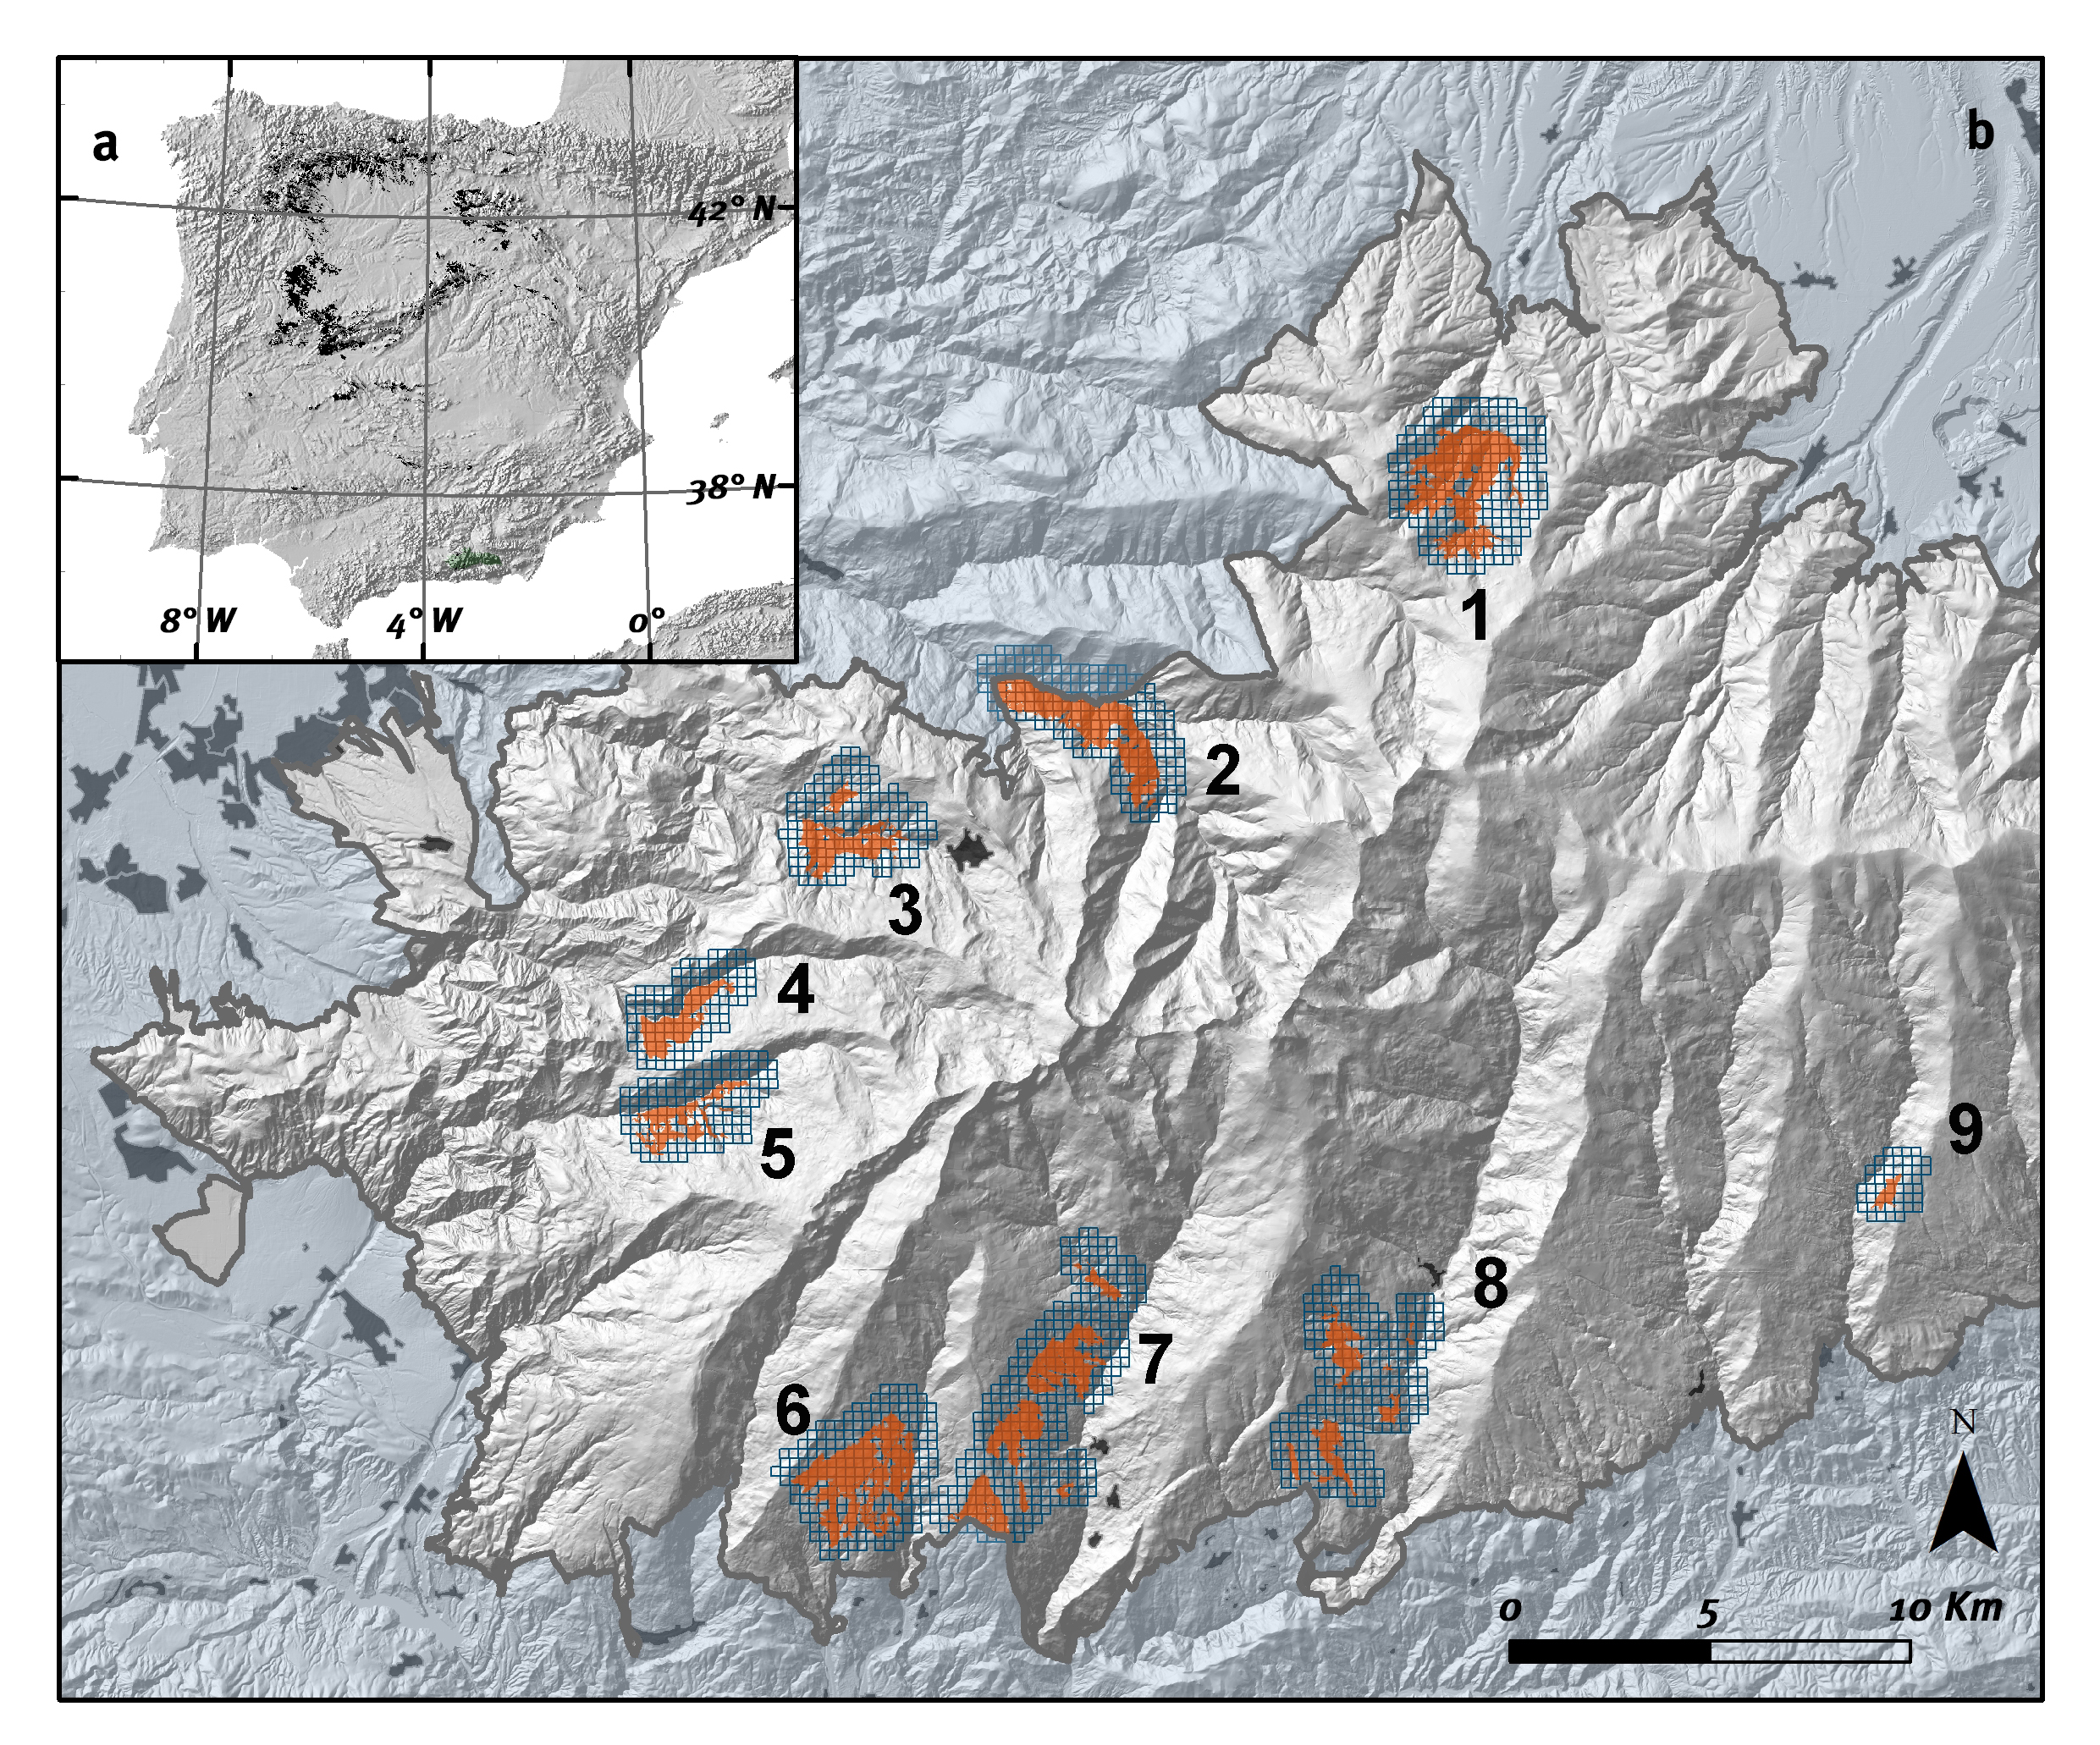
\includegraphics[width=0.7\textwidth]{img/onto/onto-location}\caption{Location of Sierra Nevada mountains. The distribution of \Qpy in the Iberian Peninsula is shown in black (\textbf{a}). The patches of \Qpy in Sierra Nevada are shown in orange (\textbf{b}). The grey line shows the boundary of the natural protected area of Sierra Nevada. The pixels used to compute the vegetation and snow indicators are included (blue grid).}\label{fig:locate}
\end{figure}

\Qpy is considered as vulnerable in southern Spain \autocite{Viveroetal2000QuercusPyrenaica} and the populations inhabiting Sierra Nevada are considered relict forests \autocite{MelendoValle2000EstudioComparativo}. They have undergone intensive anthropic use in recent decades \autocite{CamachoOlmedoetal2002AltaAlpujarra}. They are also expected to suffer the impact of climate change, due to their climate requirements (wet summers): \Qpy requires between 650 and 1200 mm of annual precipitation and minimal summer precipitation between 100 and 200 mm. Thus, simulations of the climate-change effects on this habitat point to a reduction in suitable habitat for Sierra Nevada \autocite{Benito2009EcoinformaticaAplicada,Benitoetal2011SimulatingPotential}.

\subsection{Data sets and derived information}\label{sec:onto:Data}

We have selected two MODIS products: MOD13Q1 to assess the habitat functioning and MOD10A2 to study the behaviour of an abiotic factor (snow cover). MOD13Q1 provides information on vegetation index NDVI (Normalized Difference Vegetation Index). The spatial resolution of this product is 250 m and the temporal resolution is 16 days. MOD10A2 provides information about snow cover extent \autocite{Halletal2002MODISSnowcover}. It has a periodicity of 8 days and a spatial resolution of 500 m. Each MOD10A2 pixel is labelled as snow if it has had snow on one of the previous 8 days. We selected MODIS products because both their spatial resolution and temporal resolutions are appropriate for the scope of this study.
We homogenized the different spatial and temporal resolutions in these two products to produce the final data at 500 m of spatial resolution and 16 days of temporal resolution. For the spatial resolution, we intersected the two grids to assign the identifier of any MOD10A2 pixel to its overlapping one in MOD13Q1. For temporal homogenization, we aggregated the data from MOD10A2 (8 days) to gain information regarding at least MOD13Q1 scale (\emph{i.e.} more than 16 days). We used the MODIS time series from 2000 to 2012.

NDVI seasonal measurements (aggregation of NDVI values by season) are suitable tools to quantify productivity and biomass \autocite{Runningetal2004ContinuousSatelliteDerived,Turneretal2006EvaluationMODIS}, seasonality {[}\textcite{Pineiroetal2006SeasonalVariation}; PotterBrooks1998GlobalAnalysis{]} and other phenological measurements \autocite{Clelandetal2007ShiftingPlant}. These measurements have been used to characterize ecosystem functioning \autocite{Cabelloetal2012EcosystemFunctioning}. We have calculated indicators regarding these ecological functions using the mean NDVI profiles provided by MODIS (\figref{fig:indicator}) \emph{sensu} \textcite{AlcarazSeguraetal2009BaselineCharacterization}:

\begin{itemize}
\item
  \textit{annual} and \textit{seasonal mean} (NDVI-I) which can be used to estimate fAPAR (Fraction of Absorbed Photosynthetically Active Radiation) \autocite{Sellersetal1996RevisedLand} and thus net primary production \autocite{Parueloetal1997ANPPEstimates,Sellersetal1992CanopyReflectance,Tuckeretal1985AfricanLandCover}.
\item
  \textit{annual relative range} (RREL); difference between maximum and minimum NDVI divided by annual mean. This variable provides an indicator of the seasonality of the photosynthetic activity \autocite{ParueloLauenroth1995RegionalPatterns}.
\item
  \textit{maximum} and \textit{minimum NDVI values} (MAX and MIN) and \textit{months} (MMAX and MMIN) in which they occur. They provide an additional description of phenology, indicating the intra-annual distribution of the periods with maximum and minimum photosynthetic activity \autocite{HoareFrost2004PhenologicalDescription,Lloyd1990PhenologicalClassification}.
\end{itemize}

NDSI (Normalized Difference Snow Index) is a spectral band ratio that takes advantage of the fact that snow reflectance is high in the visible wavelengths and low in the shortwave infrared region \autocite{SalomonsonAppel2006DevelopmentAqua}. This index has proven to be a robust indicator of snow cover using MODIS images\autocite{Rittgeretal2013AssessmentMethods}. We have calculated several indicators from MOD10A2 images \autocite{WangXie2009NewMethods} (\figref{fig:indicator}):

\begin{itemize}
\item
  \textit{snow-cover duration} (SCD): is defined as the number of days covered by snow per hydrological year (describe a time period of 12 months for which precipitation totals are measured).
\item
  \textit{snow-cover onset dates} (SCOD): is defined as the first date in the hydrological year that the pixel has snow. This indicator is useful to identify shifts in the starting of snow season.
\item
  \textit{snow-cover melting dates (SCMD)}: is the last date in the hydrological year that the pixel has snow. This indicator provides useful information about the melting process.
\item
  \textit{snow-cover melting cycles (SCMC)}: number of melting cycles in each pixel per hydrological year.
\end{itemize}

\begin{figure}
    \centering
    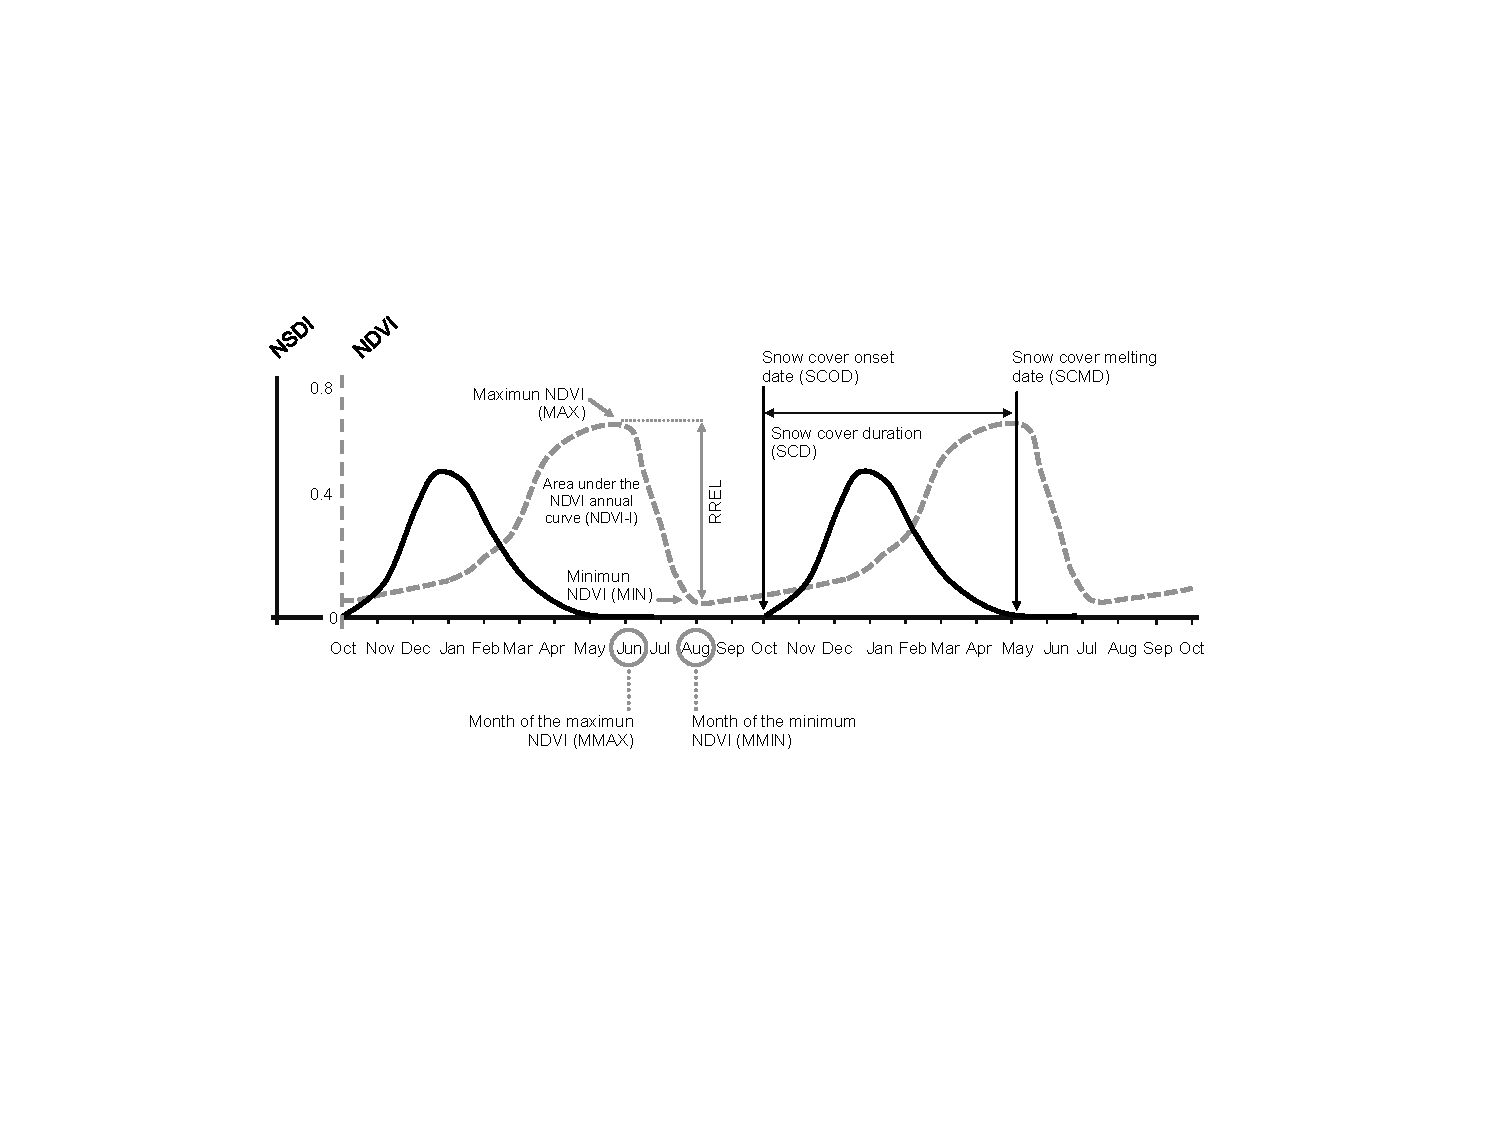
\includegraphics[width=\textwidth]{img/onto/onto-figure-indicators}\caption{Attributes derived of Normalized Difference Vegetation Index (NDVI) and snow-cover profiles. Modified from @AlcarazSeguraetal2009BaselineCharacterization and @WangXie2009NewMethods.}\label{fig:indicator}
\end{figure}

\section{Knowledge retrieval: ontologies and semantic processing}\label{sec:onto:Semantic}

Savia was designed taking into account a client-server architecture (\figref{fig:architecture}). The system contains different modules that extract relevant knowledge from the raw data. These modules act in a user-transparent way and are detailed in the following subsections, highlighting image processing, the development of the ontology, how instances are generated, and the final query system.

\begin{figure}
    \centering
    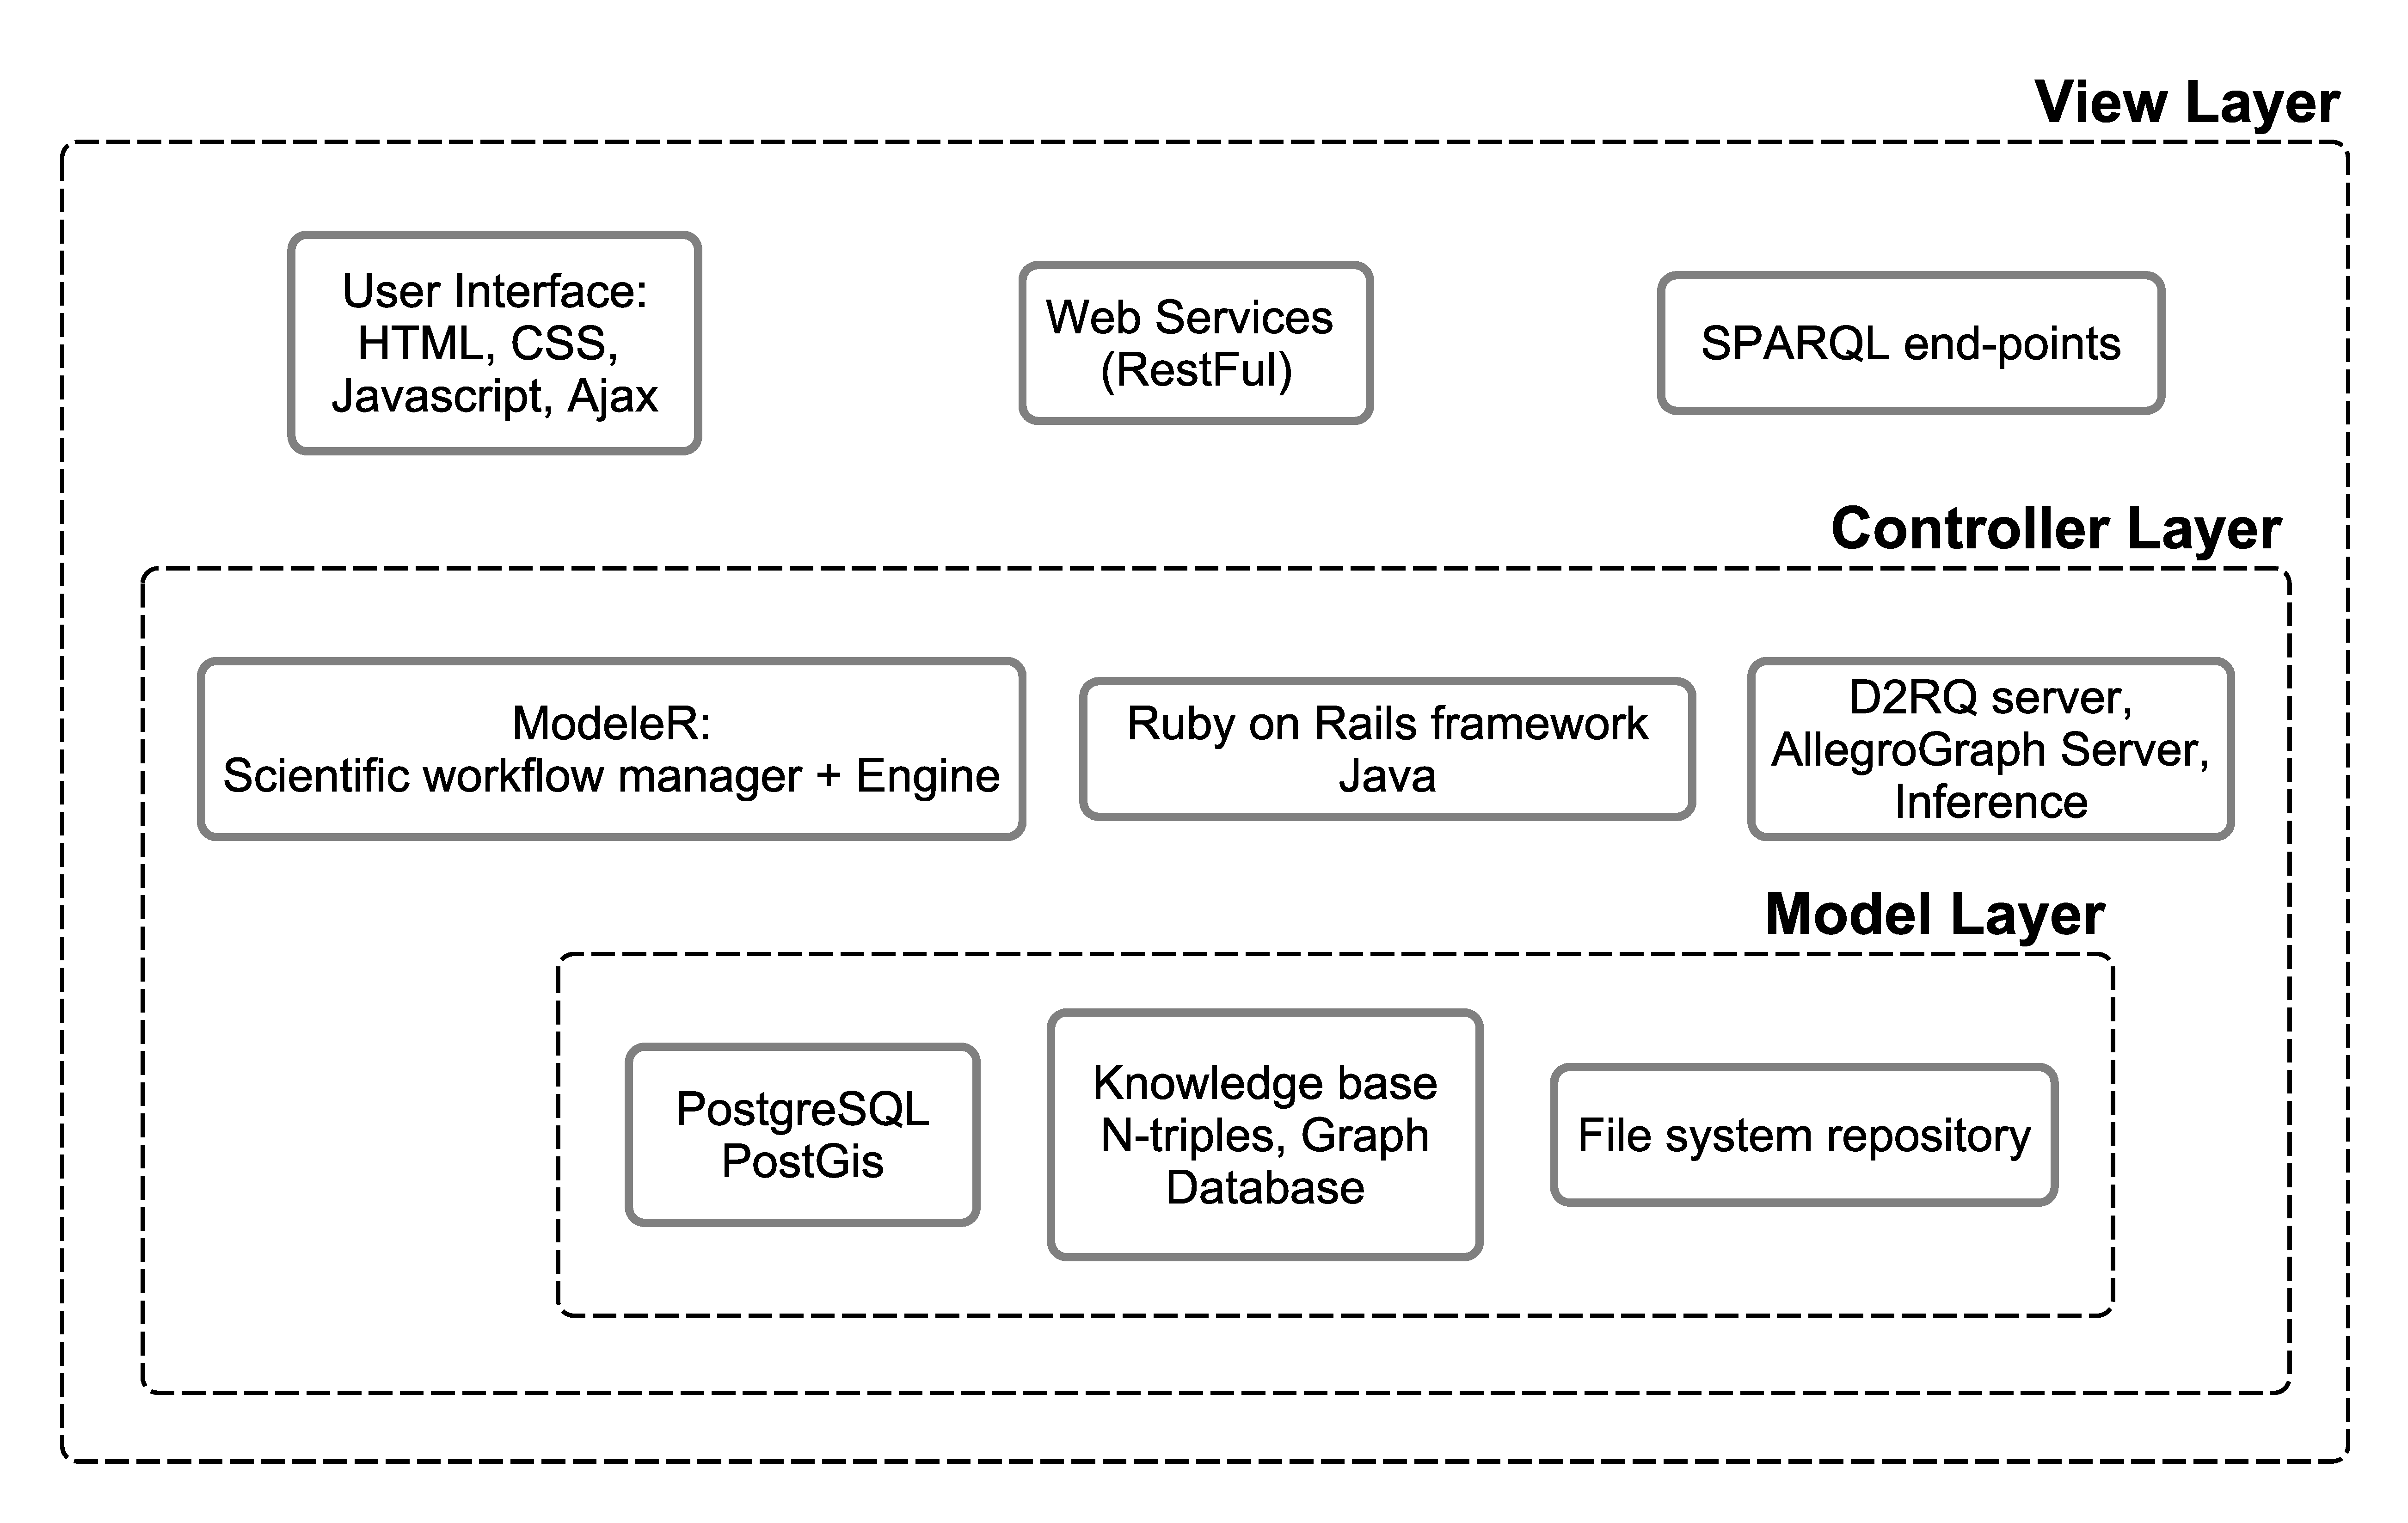
\includegraphics[width=\textwidth]{img/onto/onto-architecture}\caption{System architecture.}\label{fig:architecture}
\end{figure}

subsection{Embedding MODIS images in a database and calculating thematic indicators}\label{sec:onto:Embedding}

HDF (Hierarchical Data Format) files are downloaded from NASA servers and processed using a workflow that makes the process automatic and reproducible. This workflow is stored and documented in a model repository called ModeleR \autocite{Bonetetal2014DocumentingStoring,PerezPerezetal2012ModeleREnviromental}. The workflow extracts information contained in any HDF files and stored it in a relational database (see structure in \figref{fig:database}). NDVI and NDSI values are stored in a table that is linked to a vector layer containing the centroids of MODIS pixels. These raw data are used to aggregate and calculate the different indicators in Savia. The results are integrated again into the relational database, that is part of the Sierra Nevada LTER site information system \autocite{BonetGarciaetal2011SierraNevada}.\\
The indicators described in Section 2.2 were calculated for each pixel and temporal stage (by hydrological year, \emph{i.e.} the period between October 1st of one year and September 30th of the next; and by season) using SQL queries. The temporal trend for each pixel was calculated using the nonparametric Mann-Kendall trend test \autocite{Kendall1970RankCorrelation,Mann1945NonparametricTests}. The analyses were computed in R \autocite{RCoreTeam2013LanguageEnvironment} with Kendall package \autocite{McLeod2011KendallKendall}. We set 0.05 the alpha level for the test, and slopes with p-values \textgreater{} 0.05 were considered significant.

\begin{sidewaysfigure}
\centering
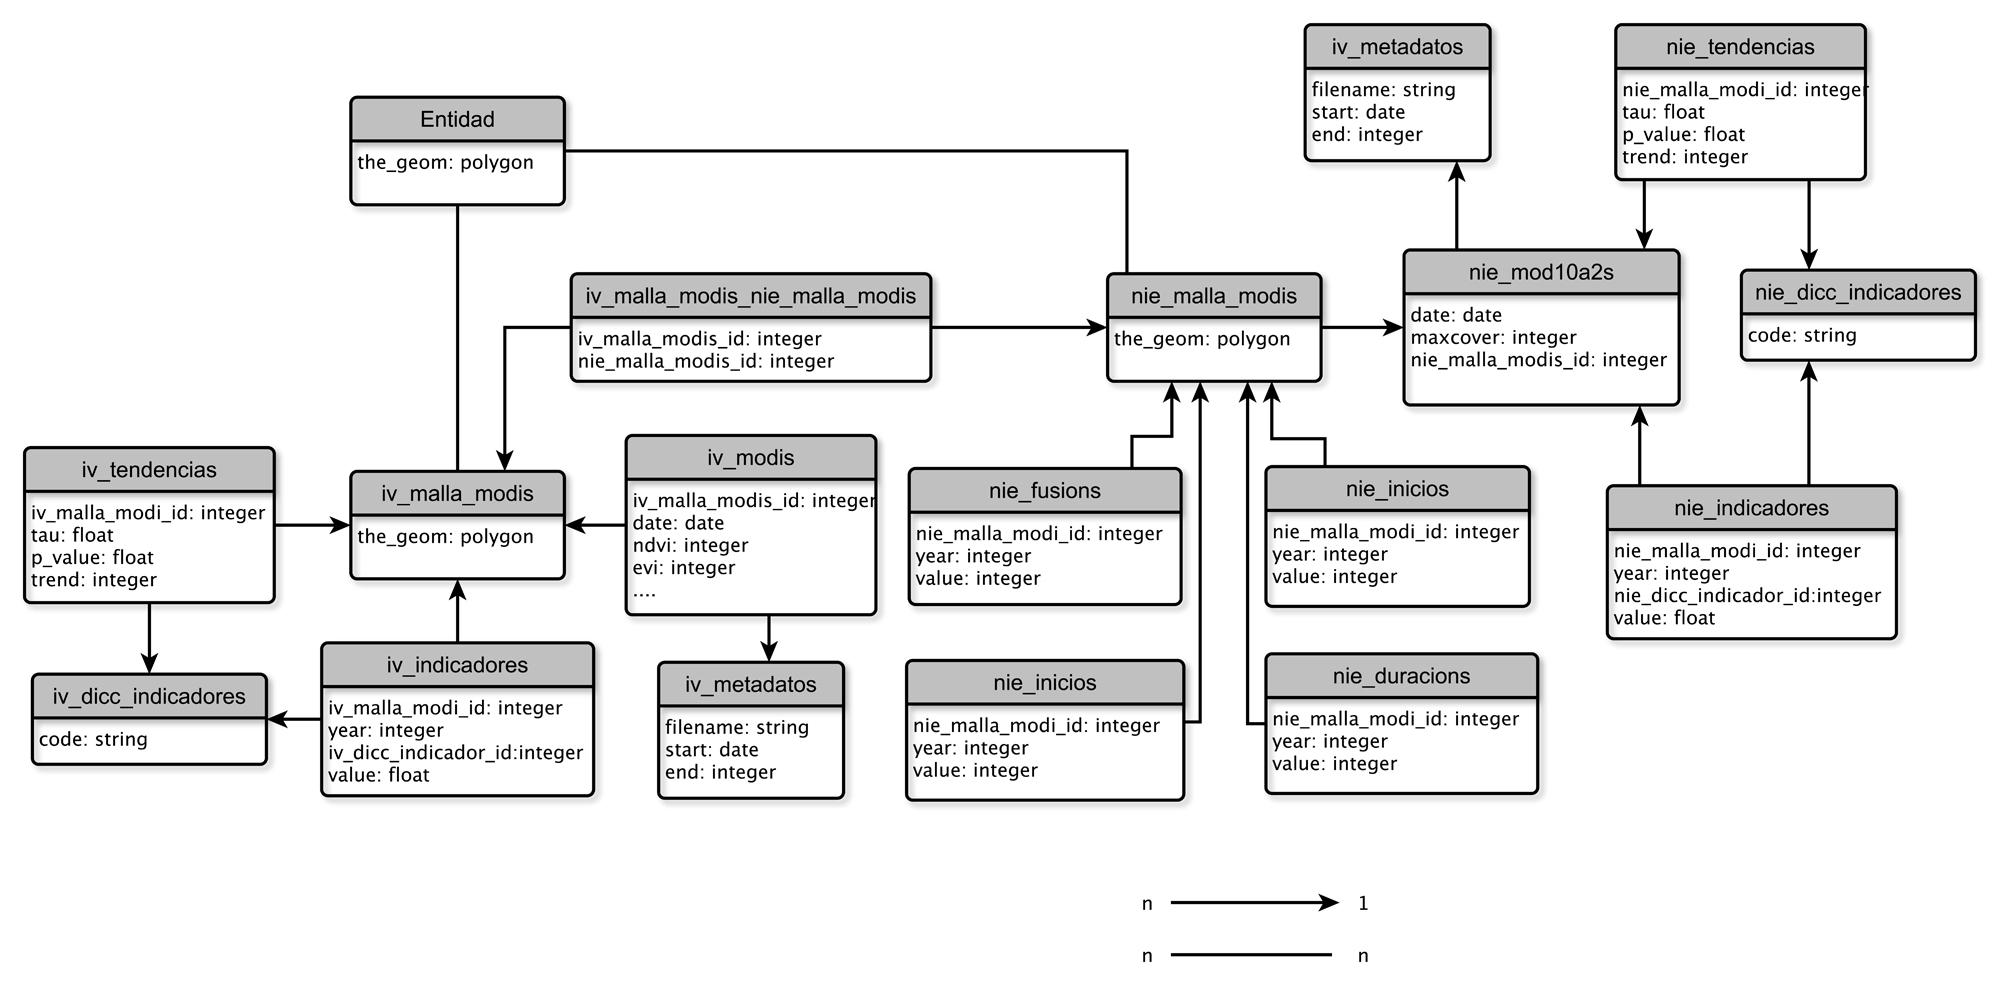
\includegraphics[]{img/onto/onto-database}\caption{Database schema. For each MODIS product the relational model stores three types of information: (i) spatial distribution of the pixels (\emph{nie\_malla\_modis} and \emph{iv\_malla\_modis} tables); (ii) values of NDVI and NDSI from original HDF files (\emph{nie\_mod10a2s} and \emph{iv\_modis} tables); and (iii) the metadata associated with each original image (\emph{nie\_metadatos\_modis} and \emph{iv\_metadatos} tables). The database also contains an auxiliary table to manage spatial entities (\emph{i.e.} \Qpy patches). Finally, there was a set of tables containing the aggregated information and indicators obtained after processing the raw data (see Section 2.2) (tables \emph{iv\_tendencias}, \emph{iv\_indices}, \emph{nie\_inicios}, \emph{nie\_fusions}, \emph{nie\_tendencias})}\label{fig:database}
\end{sidewaysfigure}

\subsection{Creating the ontology}\label{sec:onto:Creating}

The ontology must represent both the information (MODIS products, indicators, and temporal trends) and the concepts used to add ecological meaning to the data (\figref{fig:ontology}). To build the ontology, we used Time Ontology in OWL (Web Ontology Language) \autocite{HobbsPan2004OntologyTime} and Basic Geo (WGS84 lat/long) Vocabulary \autocite{Brickley2003BasicGeo} external ontologies. The OWL-Time ontology promoted by W3C (World Wide Web Consortium) \autocite{W3C2013LargeTriple}, provides a vocabulary for expressing instants and intervals, together with information concerning durations and date/time information \autocite{HobbsPan2004OntologyTime}. The Basic Geo is an RDF (Resource Description Framework) vocabulary for representing latitude, longitude, altitude information as well as other information related to spatial-located items.

Thus, the ontology takes into account three different parts (\figref{fig:ontology}):

\begin{enumerate}
    \item Representing spatial information. The main concept is the Pixel, which represents a pixel from a MODIS image. Some pixels that share similar functions (\emph{i.e.} be covered by the same habitat) may belong to a Patch. Finally, some patches sharing the same dynamics may belong to a Group. The properties called \emph{PixelBelongsToPatch} and \emph{PatchBelongsToGroup} help to define the relationships between the previously defined concepts. \emph{PixelIsNearTo} is another useful property that adds the functionality of proximity to any pixel. The distance threshold used was 500 m between pixels (500 m is the spatial resolution of MODIS snow products). This property is symmetric because when a pixel A is near B, B is also near A.
    \item Indicators. This part contains a concept (\emph{IndicatorValues}) that represents the different values that take an indicator (see Section 2.2) at a given time point (through the concept called time: Year and the property \emph{HasYear}) and in a given place (through the concept Pixel and the property \emph{IndicatorValuesLocateInPixel}). We have also included a concept to describe all the indicators (Snow-cover duration, Snow-cover onset date, NDVI\_i annual, Maximum NDVI, etc.). These concepts are grouped according to their thematic area (Snow and Vegetation). Each indicator has a property called value that is measured using a given specific unit.
    \item The temporal trends are described in a concept called \emph{IndicatorTrend}. This concept shows the temporal trend of a single point for the whole time series (it is linked to \emph{Pixel} via \emph{PixelHasIndicatorTrends}). We have also created a concept for each temporal trend calculated for the previously described indicators (Trend of Snow cover duration, Trend NDVI\_i annual, etc.). These concepts are also grouped according to their thematic area (Snow Trend, Vegetation Trend). All these concepts have the following properties:
    \begin{enumerate}
        \item \emph{value\_tau} and \emph{p\_value}: These properties contain the statistic (\emph{value\_tau}) and the significance (\emph{p\_value}) reached by the Mann-Kendall trend analysis.
        \item \emph{value\_trend}: Categorical property ranges from -1 (significant negative trend) to 1 (significant positive trend). It is calculated according to the values of \emph{value\_tau} and \emph{p\_value.}
    \end{enumerate}
\end{enumerate}

This schema was implemented using OWL DL (Description logic) that allows an enhanced expression level and does not limit the values for cardinality \autocite{Smithetal2004OWLWeb}. The structure of the ontology created can be downloaded following this link: \url{http://iecolab.es/indicators.rdf}

\begin{sidewaysfigure}
\centering
    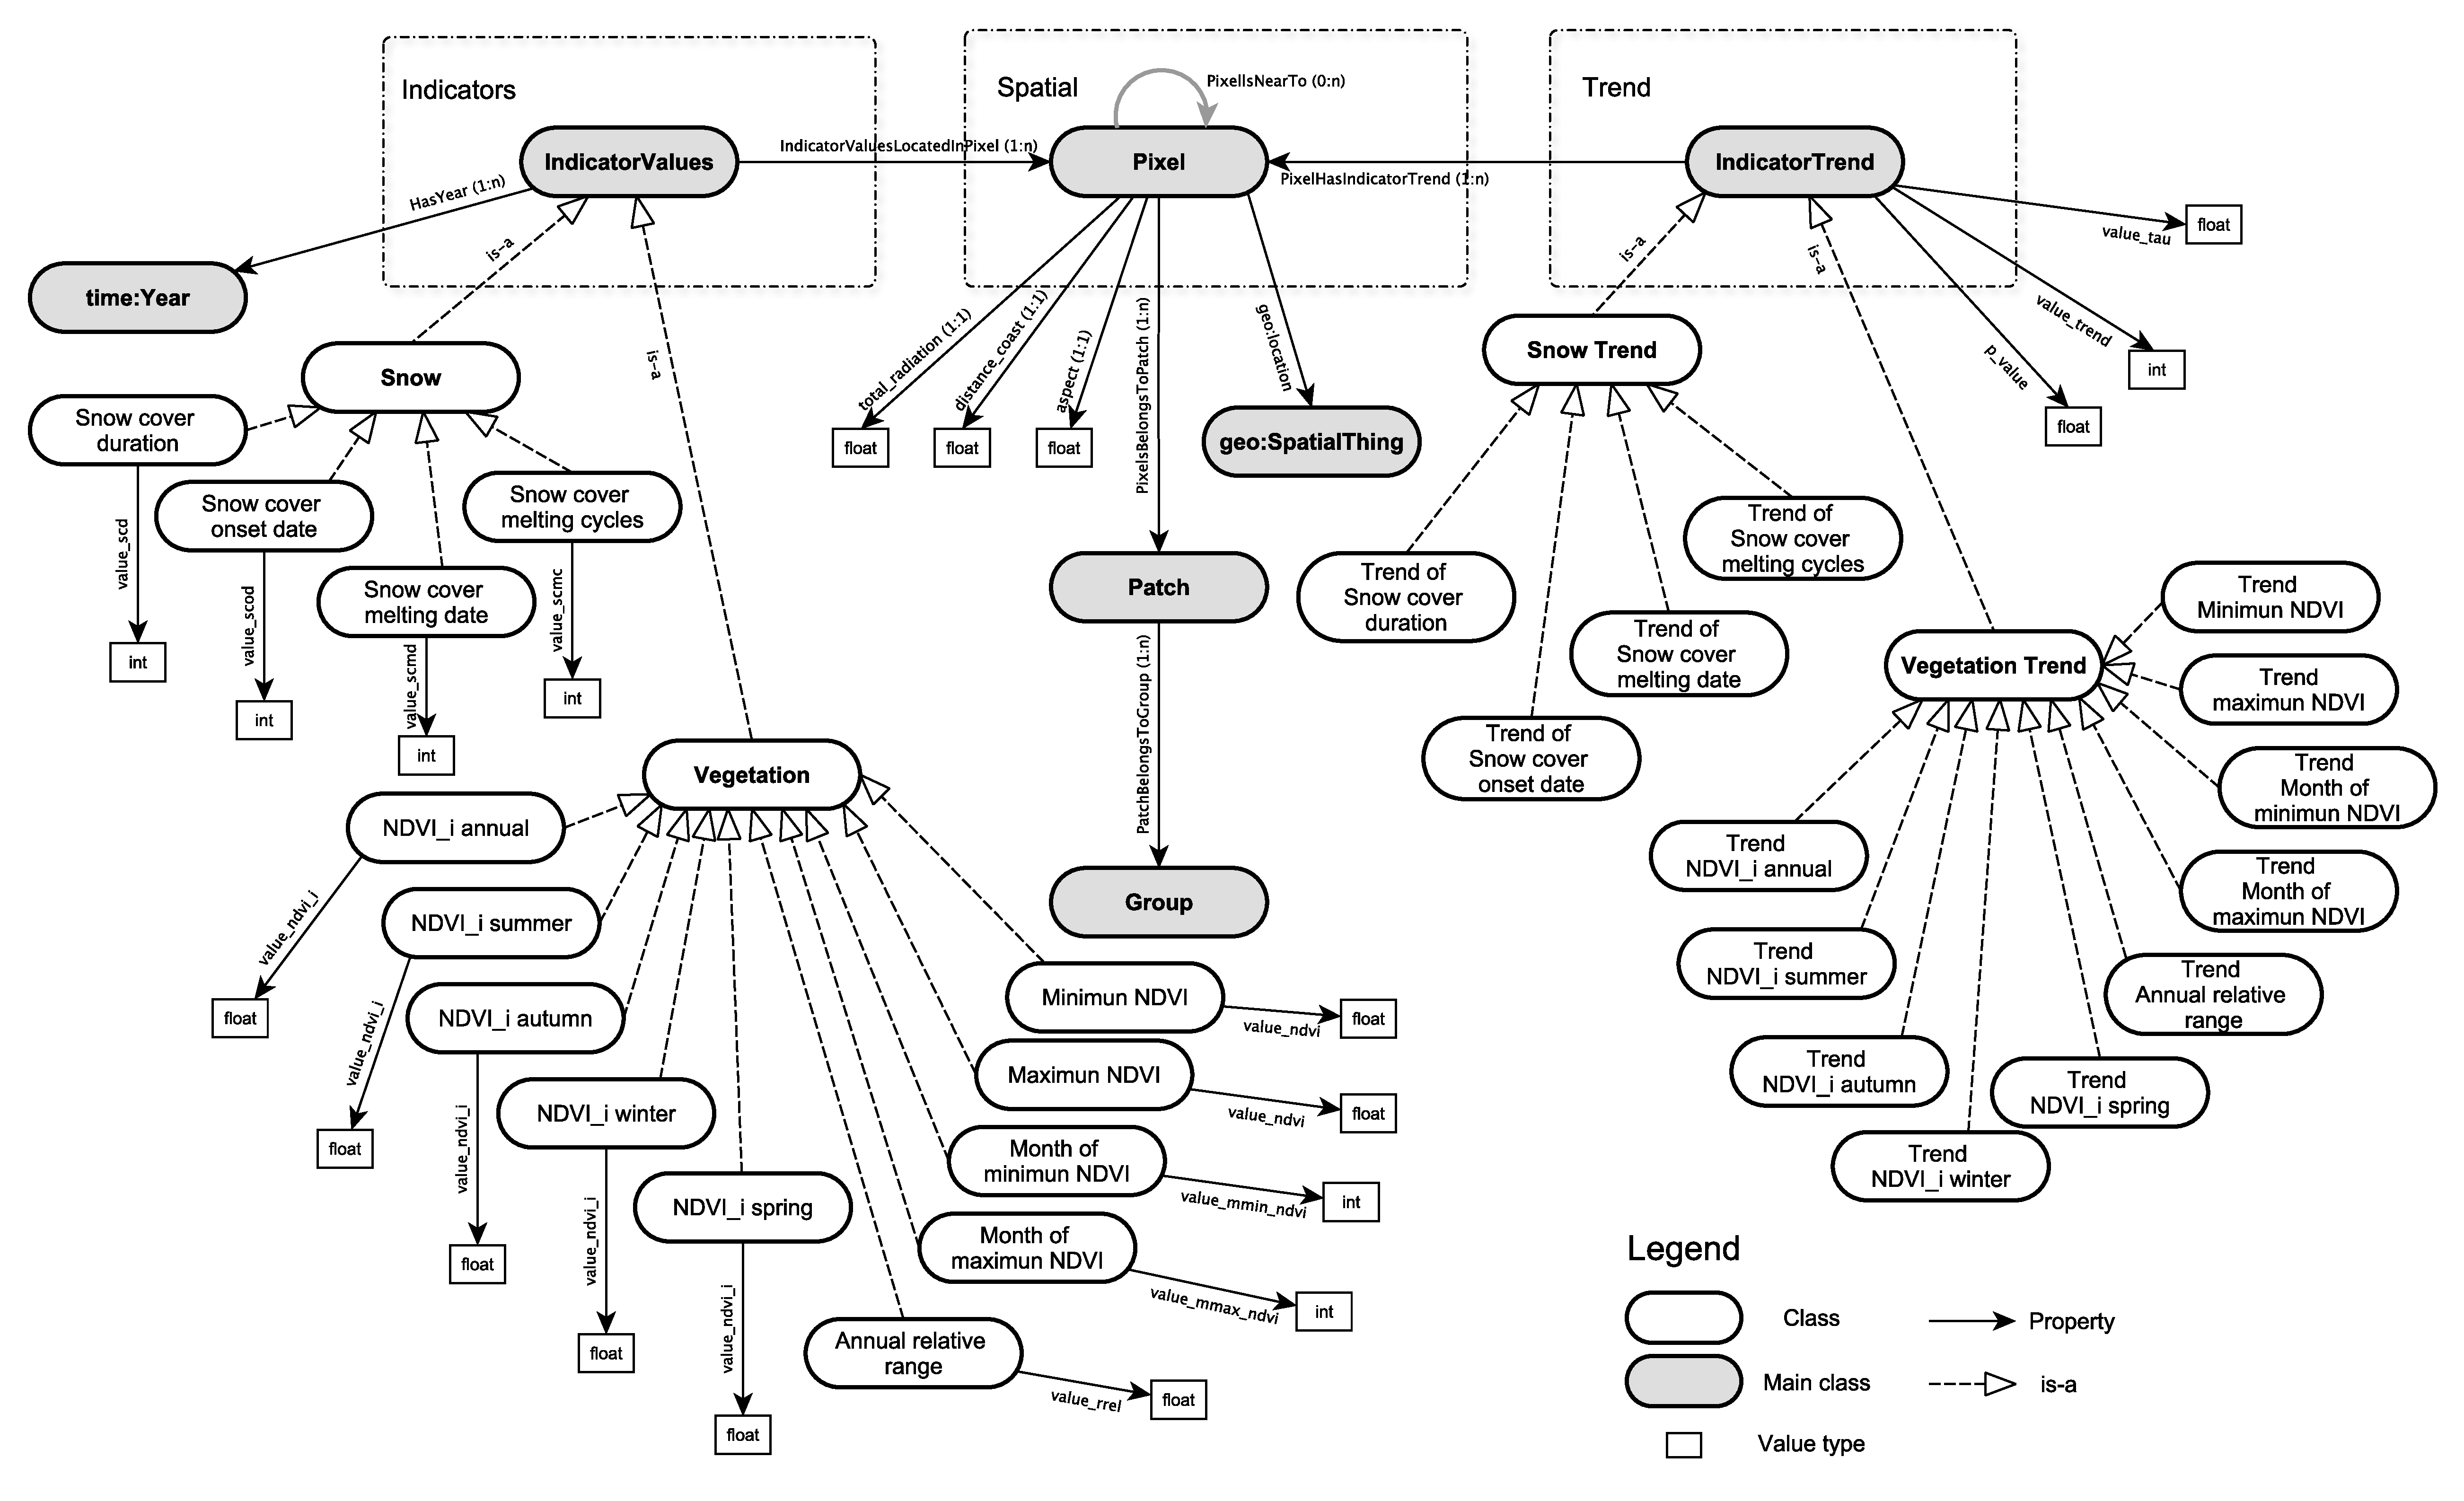
\includegraphics[width=\textwidth]{img/onto/onto-ontology}\caption{Detailed representation of the ontology created. Three main parts are considered:  spatial information, indicators, and temporal trends of the indicators}\label{fig:ontology}
\end{sidewaysfigure}

\subsection{Knowledge base, SPARQL endpoint and inference}\label{sec:onto:SPARQL}

The next step after creating the ontology is to map the records in the database that contain the data to the ontology. Firstly, we used D2RQ \autocite{Bizeretal2004D2RQTreating} to map the relational database to OWL ontology. This software allows instance data to be retrieved from relational databases on-the-fly during the execution of SPARQL queries. Nevertheless, this procedure is time consuming and demands powerful computational capabilities. Thus, we dumped the mapping created with D2RQ into an intermediate N-triples file to avoid this drawback \autocite{Sarkaretal2011LinkedData}. This file was created with the data existing in the database and has all the triplets contained in the knowledge base.

To store the knowledge base, our tests with the open-source Apache Fuseki and Jena (\url{http://jena.apache.org/}) frameworks yielded unsuccessful results as soon as the data volume started to grow. Because we need an efficient implementation that can be scaled to large, enterprise-class data \autocite{Wilkinsonetal2004EfficientRDFa}, we also conducted some tests with AllegroGraph (\url{http://www.franz.com/agraph/allegrograph/}) and Virtuoso (\url{http://virtuoso.openlinksw.com/}), choosing the former option because of its capabilities and user-friendly management environment. This software is a triplestore that uses a graph database and it has the ability to encode values directly into its triples.
To enhance the results of the queries, a reasoning task can be also triggered within the generation of the system output process. AllegroGraph provides a built-in inference engine that derives implicit information from the knowledge base. Thus, users can easily turn it on by toggling that option in the query builder interface to enrich their queries. The inference engine is useful to find relations on different types of indicators and other implicit properties such as \emph{PixelIsNearTo}. For example, Savia can answer questions concerning implicit knowledge of pixels with a positive trend on seasonal mean of NDVI near others with a negative trend in snow-cover melting dates.

\section{Study Case}\label{sec:onto:CaseStudy}

For the improvement of the conservation status of habitats, it is necessary to implement management plans according to the Annex 6 of the Habitats Directive. Our system provides knowledge useful to design those management plans. We have used \Qp forests in Sierra Nevada (Spain) to explore the importance of snow duration in the functioning of \Qp forests. We have chosen this habitat as a case study for two reasons: \emph{a)} its interesting ecological dynamics (deciduous forest in a Mediterranean mountain), and \emph{b)} the need to manage these forests in a global-change context.

We have structured the case study according to three questions that will provide two types of results. Some of them will help in the understanding of the ecological functioning of the target habitat. And others will demonstrate how ontologies are useful tools to make remote sensing information more accessible for non-expert users.

\subsection{Which pixels show a trend towards higher productivity in summer?}\label{sec:onto:Trends}

\Qp forests show a well-defined growth season centred in summer \autocite{Alcarazetal2006IdentificationCurrent,Dionisioetal2012SatelliteBasedMonitoring}. Some works have pointed out changes in habitat functioning: increase in annual vegetation greenness in Sierra Nevada \autocite{AlcarazSeguraetal2008TrendsSurface,AlcarazSeguraetal2010EvaluatingConsistency} and seasonal functional changes in \Qp woodlands \autocite{Marty2008RegimeShift}, during the last decade.

This question aims to explore whether our target habitat is undergoing changes in summer productivity, specifically which \Qp forests of Sierra Nevada have shown a positive trend of the value of summer productivity (summer NDVI).

\begin{sidewaysfigure}
\centering
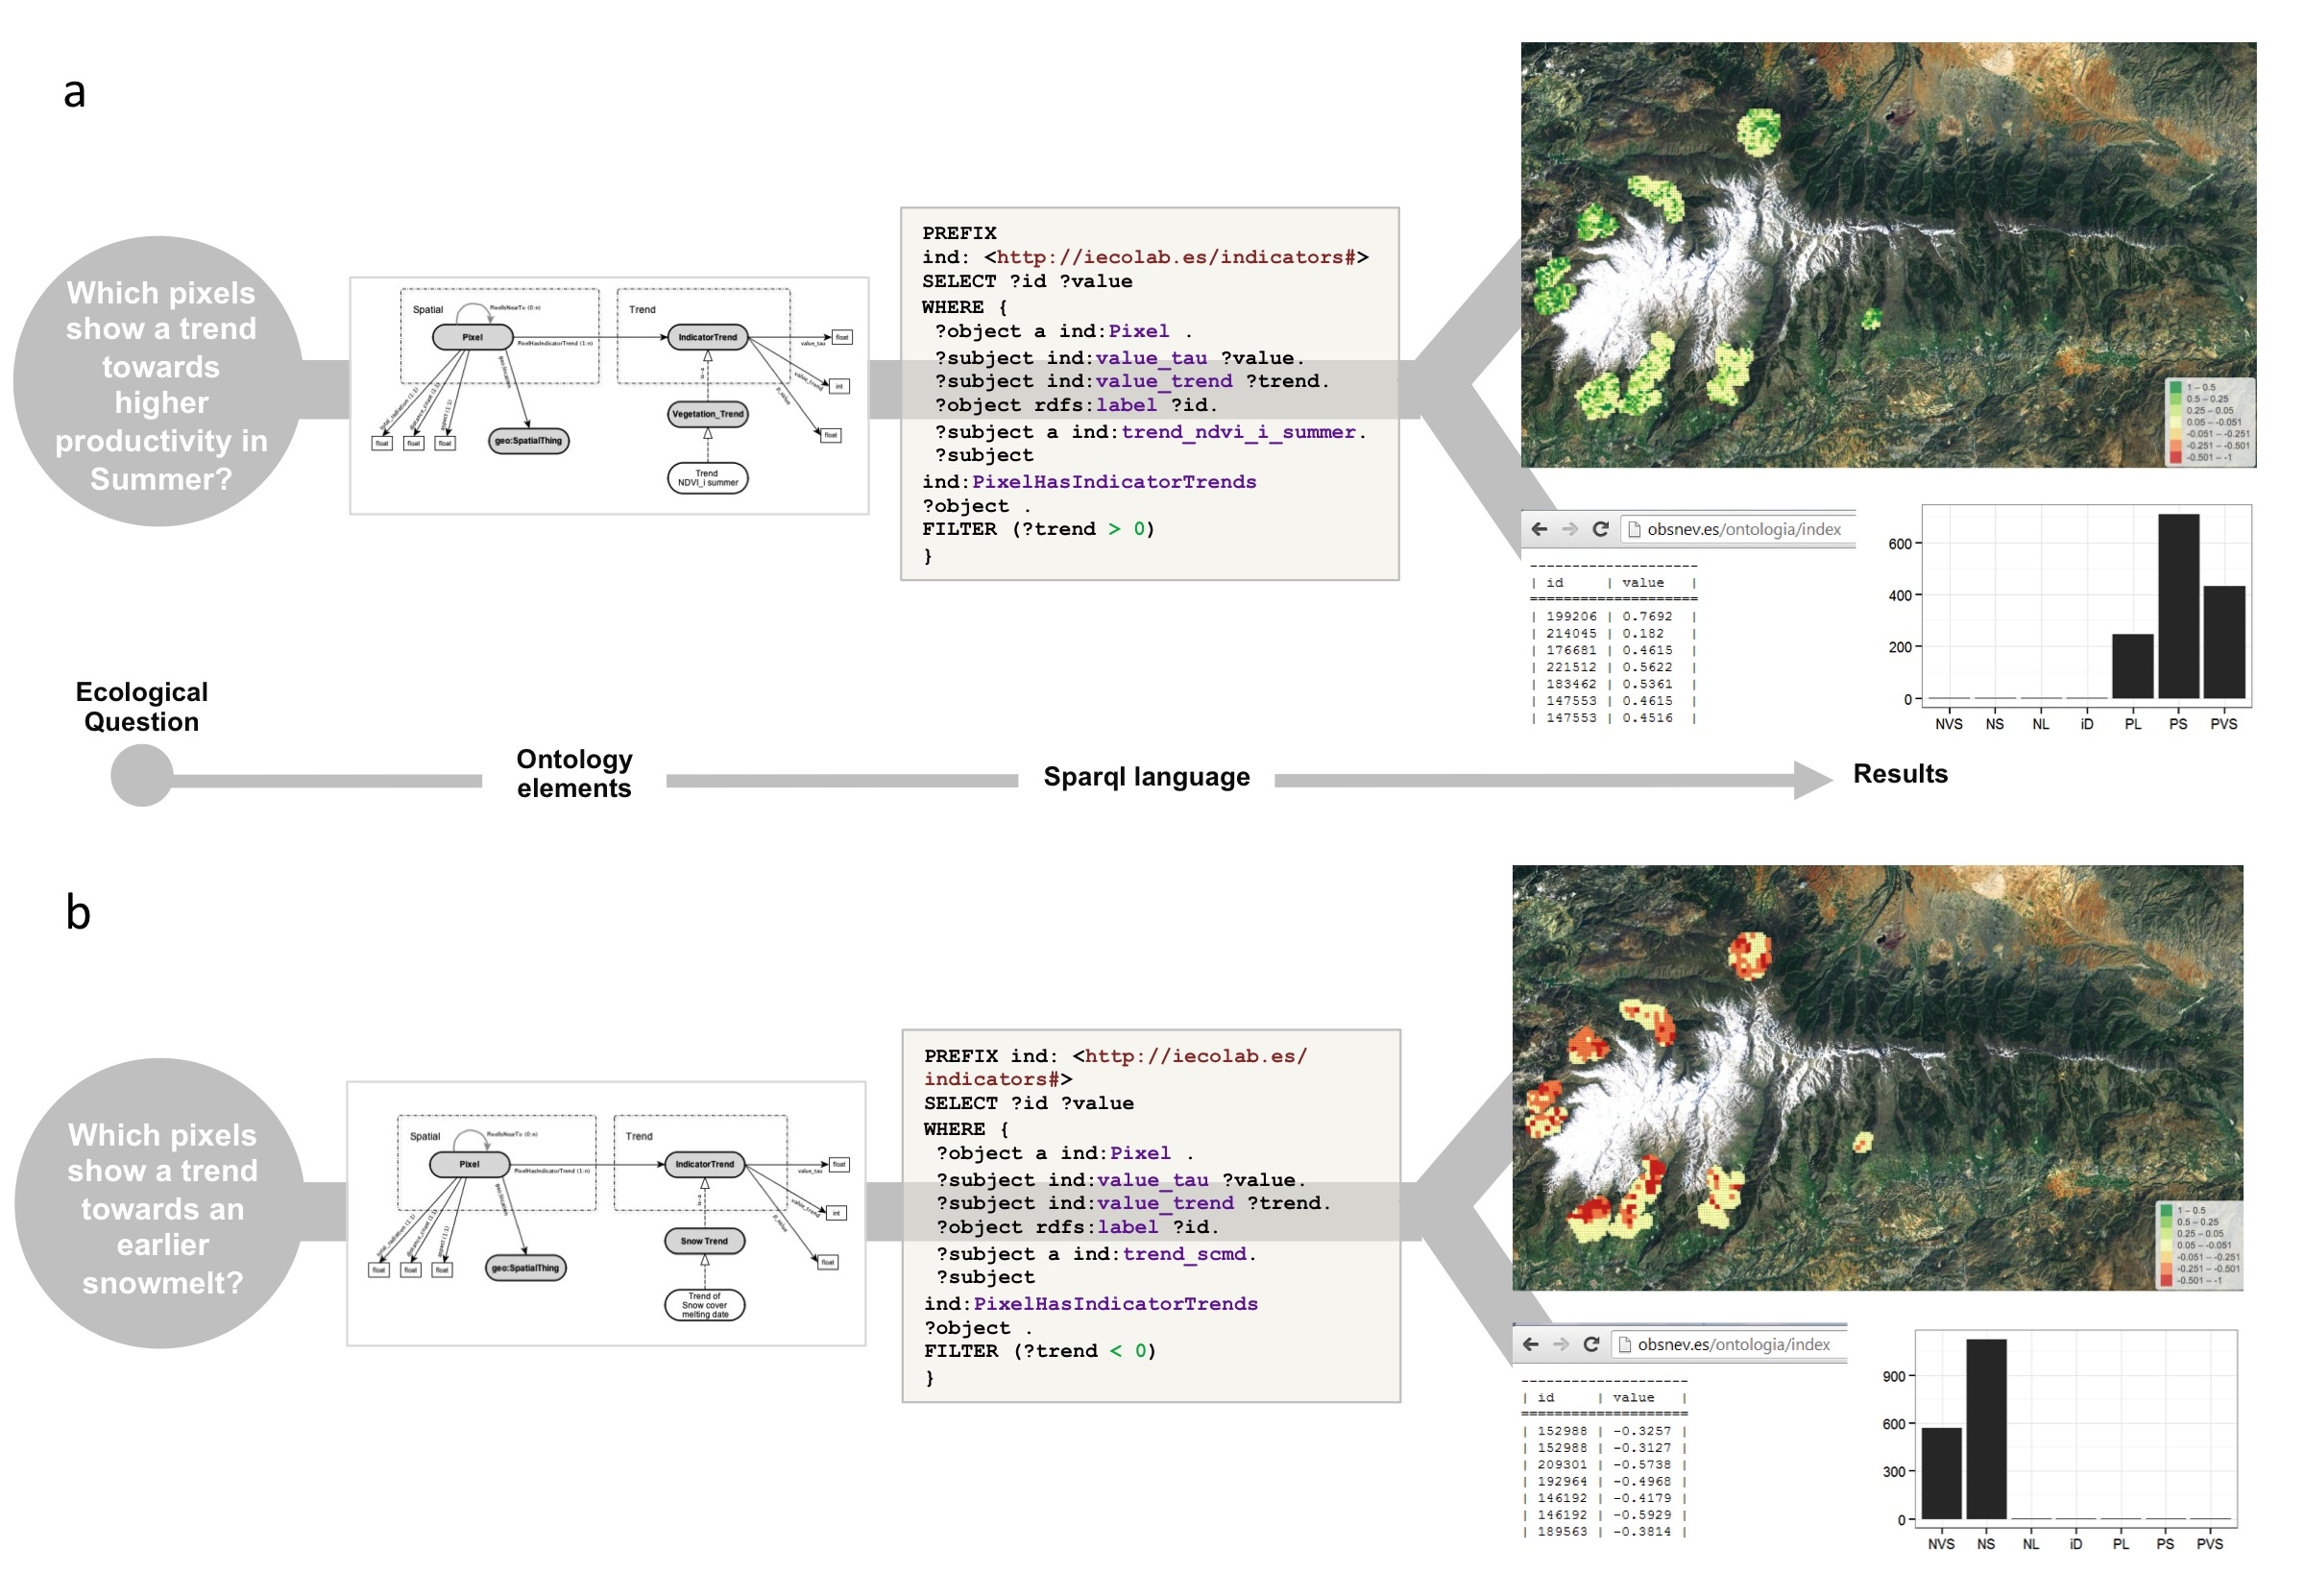
\includegraphics[width=.8\textwidth]{img/onto/onto-case-study}\caption{Scheme showing how the ontology solves questions regarding habitat functioning (a) and the behaviour of an abiotic factor (b). For each ecological question, different ontology elements are used to answer it. Then SPARQL language is used to query the knowledge base. Finally, results can be shown in different formats: map, csv or histogram. See first and second question of the study case. All pixels are displayed on the resulting map, but for those that have a significant positive trend the tau value is retrieved. In the map, we show seven different colours corresponding to this classification of tau values: [1, 0.5], [0.5, 0.25], [0.25, 0.05], [0.05, -0.051], [-0.051, -0.251], [-0.251, -0.501], [-0.501, -1].}\label{fig:casestudy}
\end{sidewaysfigure}

\subsection{Which pixels show a trend towards an earlier snowmelt?}\label{sec:onto:Snowmelt}

Several studies have pointed out a trend towards higher temperatures and lower precipitation for the Mediterranean area \autocite{GarciaRuizetal2011MediterraneanWater,GiorgiLionello2008ClimateChange}. Significant declines in snow-cover extent and duration has been reported in some European mountains \autocite{Marty2008RegimeShift,MorenoRodriguezetal2005EvaluacionPreliminar,Nikolovaetal2013ChangesSnowfall,Scherreretal2004TrendsSwiss}. Climate projections forecast an increase of +4.8ºC at the end of the 21st century \autocite{Benitoetal2011SimulatingPotential} for Sierra Nevada and it expected that snowmelt will occur earlier in the year and will be more rapid \autocite{GarciaRuizetal2011MediterraneanWater}.

The second question that we raised it concerns the observed changes in snowpack in Sierra Nevada. We are interested specifically in which pixels show a trend towards earlier snowmelt during spring-summer. This question is crucial, given that \emph{Q. pyrenaica} forests need water in summer for growth.

\subsection{Which \emph{Q. pyrenaica} patches show a trend towards a more productive summer and earlier snowmelt?}\label{sec:ontoProductive}

This question explores the relationships and co-occurrence between biological production and snow-cover features.

Snow-related variables can explain the distribution of plant communities in the landscape \autocite{Jonesetal2001SnowEcology}. This causal relationship is more important at high elevation \autocite{BonetGarciaCayuela2009SeguimientoCubierta} in Sierra Nevada. But snow cover also explains part of the ecosystem functioning. \textcite{Trujilloetal2012ElevationdependentInfluence} that vegetation greenness increases with snow accumulation. This relationship varies with elevation, reaching a maximum between 2000-2600 m.

Some works have pointed out the influence of snow on greenness in Pyrenean oak forests \autocite{AlcarazSeguraetal2009BaselineCharacterization,Dionisioetal2012SatelliteBasedMonitoring}, but to date we have found no studies that analyse the coupling between snow cover and forest greening. Water availability is a key issue on the distribution of \emph{Q. pyrenaica} \autocite{delRioetal2007BioclimaticAnalysis,Gavilanetal2007ModellingCurrent}. This combination of plant growth and water scarcity makes summer a critical season for the functioning of this habitat.

The third question assesses the capacity of our ontology to show relationships similar to those described above. We have explored the co-occurrence of significant trends in biological production and snow-cover melting date in \emph{Q. pyrenaica} forests. In other words, we have analysed which \emph{Q. pyrenaica} forests show a trend towards higher productivity and earlier melting date in summer.

\section{Results}\label{sec:onto:Results}

We translated the above questions from natural language into ontology. For the first and second questions (Sections 4.1 and 4.2) we used two concepts (\emph{Pixel}, \emph{IndicatorTrend}) and some properties describing these concepts (\emph{value\_trend}, \emph{value\_tau}, \emph{PixelHasIndicatorTrends}, \emph{Trend NDVI\_i summer}, \emph{Trend of Snow cover melting date}) included in the ontology. Specifically:

\begin{itemize}
\item
  \emph{``select all Pixel where IndicatorTrend is positive for summer NDVI-I indicator''} for question 4.1 (\figref{fig:case-study}a)
\item
  \emph{``select all Pixel where IndicatorTrend is negative for snow-cover melting date''} for question 4.2 (\figref{fig:case-study}b)
\end{itemize}

We used SPARQL language to query the knowledge base.

Regarding the first question, we found that 75\% of pixels had a positive significant trend for summer NDVI (\figref{fig:casestudy}a). For these, more than 80\% showed a strong or very strong positive trend. In general, \emph{Q. pyrenaica} patches located on the north face of Sierra Nevada showed a higher amount of significant pixels than the southern ones did (see map in \figref{fig:case-study}a).

The second question showed that almost 70\% of the pixels covered by \emph{Q. pyrenaica} forests had a strong or very strong negative and significant trend towards an earlier melting date (\figref{fig:casestudy}b). Similar to NDVI, the northern patches showed a higher amount of significant pixels than the southern ones.

The third question is more difficult to translate to the ontology because it takes into account two datasets and more concepts than the previous questions. We have included a concept called Patch, being a subset of pixels that share some ecological features (they belong to the same \emph{Q. pyrenaica} population). This question also includes other concepts already mentioned (\emph{Pixel}, \emph{IndicatorTrend}) and properties describing those concepts (\emph{value\_trend}, \emph{value\_tau}, \emph{PixelHasIndicatorTrends}). We also calculated the percentage of pixels per Patch that showed trends towards more productive summers and earlier snowmelt. These elements were used to translate the original question to another one that was more suitable for the ontology: select all Pixels where the \emph{IndicatorTrend} is positive for the summer NDVI-I indicator (\emph{Trend NDVI\_i summer}) and negative for snow-cover melting date (\emph{Trend of Snow-cover melting date}). We used SPARQL language to query the knowledge base. The results can be displayed both in a map and table format (\figref{fig:casestudyQ3}).

Savia provides two types of answers for this question: \emph{a)} A table (\figref{fig:case-studyQ3}) shows the different \emph{Q. pyrenaica} patches ranked according to the percentage of pixels having the described trends in summer productivity and snow-cover melting date. \emph{b)} A binary map showing the pixels (grouped by \emph{Patch}) that satisfy both conditions (\figref{fig:case-studyQ3}). All the patches that share the same behaviour are considered as Groups.

\section{Discussion and Conclusions}\label{sec:ontoDiscussion}

The system that we have created adds a semantic component to remote-sensing images using ontologies to describe this information. Savia is an operational system that is available for any user via the web (\url{http://obsnev.es/ontologia/index}).
Our system implements a query builder user interface that allows users to build questions using SPARQL. It also includes a set of predefined questions to show its capabilities. Furthermore, users can select different output file formats to display results (csv, text or map). All the analytical procedures needed to run this system have been documented using a model repository called ModeleR \autocite{Bonetetal2014DocumentingStoring,PerezPerezetal2012ModeleREnviromental}. The ontology created reuses and extends public ontologies like OWL-Time and Basic Geo (WGS84 lat/long) Vocabulary. The database containing MODIS images was translated into facts within a knowledge base. This requires a mapping between the database and the concepts contained in the ontology. The dynamical queries to knowledge base, using the mapping tool, were one of the most relevant bottlenecks that we have found during the implementation of the system, and we finally used enterprise-ready software to optimise queries to the knowledge base. We also used an inference engine to solve complex queries that require using advanced properties in the ontology (transitivity and symmetry, mainly).

We tested the ontological system in a case study focusing on \emph{Q. pyrenaica} habitat in Sierra Nevada. We identified significant trends in summer NDVI for 75\% of pixels covered by the target habitat. These pixels were located mainly in northern-faced patches (aspect was calculated using DEM). These results could be explained by a different pattern of summer productivity among the \emph{Q. pyrenaica} patches. We have also described similar trends in snow patterns: 70\% of pixels show a significant and negative trend towards an earlier melting date. Most of those pixels are also located in northerly facing patches. This result could have several hydrological and ecological implications: a) water from the melted snow is available for vegetation earlier each year, which could help deciduous trees to overcome the summer drought, b) the ground is free of snow during a longer period each year, which could provide extra area to treeline communities for altitudinal shifts.

The ontology has also helped to unveil the co-occurrence of significant trends both in snow cover (abiotic factor) and ecosystem functioning (NDVI). Thus, western patches display a high percentage of pixels showing this co-occurrence. The ecological implications of this co-occurrence can be explained by arguing that the earlier snowmelt provides water to \emph{Q. pyrenaica }trees when they are in the middle of their growing season. This earlier amount of water supply encourages trees to be more productive in summer. On the other hand, the southern patches also show this co-occurrence in the opposite way: The lack of significant trends in summer productivity for southern patches could be explained by the lack of pixels with trends towards earlier snowmelt in these areas. Although these results are still preliminary, we have established a link between the status of an abiotic factor and the functioning of ecosystems. Some forest activities can be scheduled according to the trends observed. It could be useful, for example, to reinforce the western patches by planting \emph{Q. pyrenaica} trees. These new trees could take advantage of the productive summers in order to create denser forests. These ecological results are similar to others found in different habitats (Trujillo et al.~2012).

The results (both ecological and methodological) demonstrate that the information in the MODIS time series is useful to assess the functioning of a terrestrial Natura 2000 habitat. We have described the temporal behaviour of \emph{Q. pyrenaica} forests in Sierra Nevada, distinguishing among patches located in areas with different environmental conditions. We have also showed temporal trends in several functioning indicators. The trends discovered would help managers to assess the conservation status of this habitat. They can also build management plans using the knowledge provided by our ontology (\emph{i.e.} to decide where to locate plantations taking into account the productivity trends). We have also described the behaviour of a key abiotic factor: snow cover; and we calculated trends for several snow-cover related indicators (snow duration, snow-cover melting date, etc.). Those could help managers to identify places where snow-cover trends could change in the coming years. Finally, we have detected relationships between trends in habitat productivity and snow-cover melting date for the target habitat. All this knowledge is offered to users (mainly managers and scientists) through a web portal, the use of which does not require expertise in remote sensing. Thus, we believe that this work is a worthwhile example of a web-based expert system created using an interdisciplinary approach.

\begin{figure}
\centering
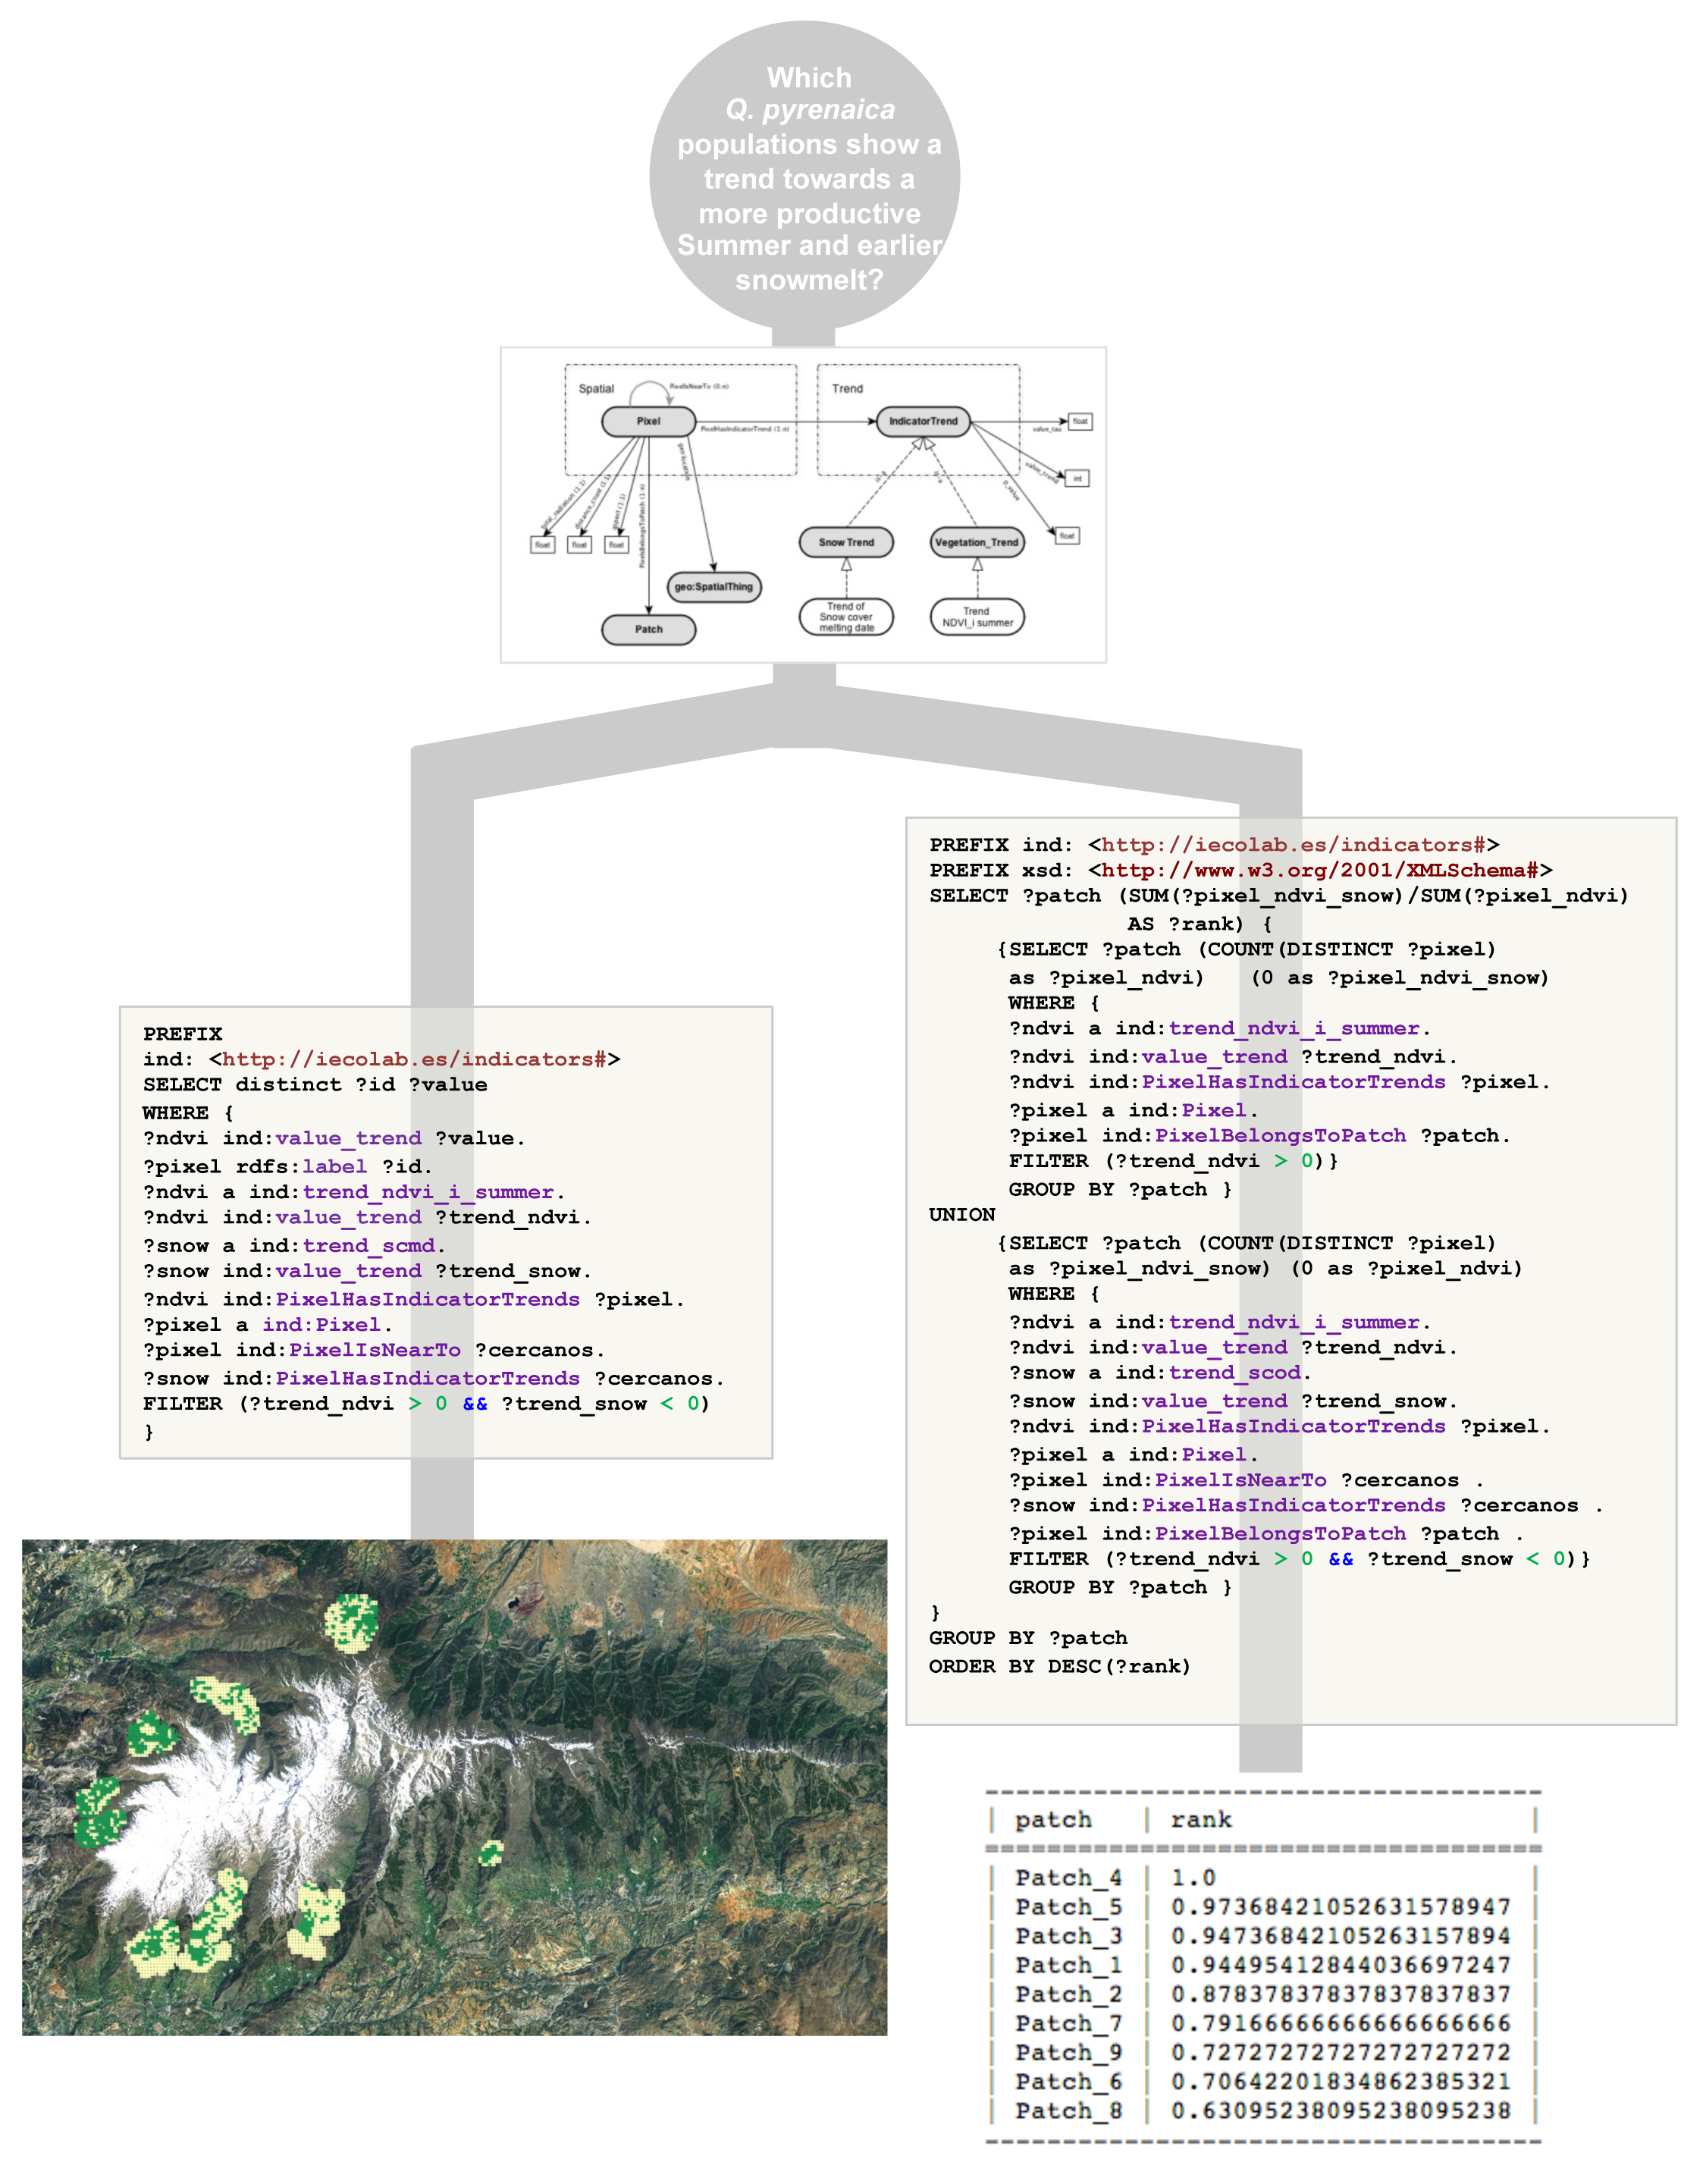
\includegraphics[width=\textwidth]{img/onto/onto-case-studyQ3.jpg}\caption{Scheme showing the process of answering a complex query by the ontology. The question takes into account trends in habitat functioning as well as trends in snow-cover melting date. We first show the concepts used by the ontology to answer the query, then the SPARQL code and finally the results found. The left branch provides a map showing those pixels with trends towards more productive summers and earlier snowmelt date. The right branch offers a table ranking the Pyrenean oak patches according to the percentage of pixels that satisfies both conditions.}\label{fig:casestudyQ3}
\end{figure}